
% Capítulo 5. Instrumentos giroscópicos
% 5.1.       Propiedades giroscópicas aplicadas al instrumental aeronáutico de a bordo.
% 5.2.       Indicadores de virajes, neumáticos, de CC y CA .
% 5.3.       Indicadores de actitud en dos ejes con giróscopo integrado, y remoto.
% 5.4.       Magnetismo terrestre, brújula, giróscopo direccional libre.
% 5.5.       Compás giroscópico auto-corregido, indicador con giróscopo integrado, y remoto.
% 5.6.       Central giroscópica para la indicación de actitud en tres ejes y toda actitud.
% 5.7.       Giróscopo LASER


\chapter{Instrumentos girosc\'opicos}
\label{sec:instrumentos.giroscopicos}



\begin{landscape}

  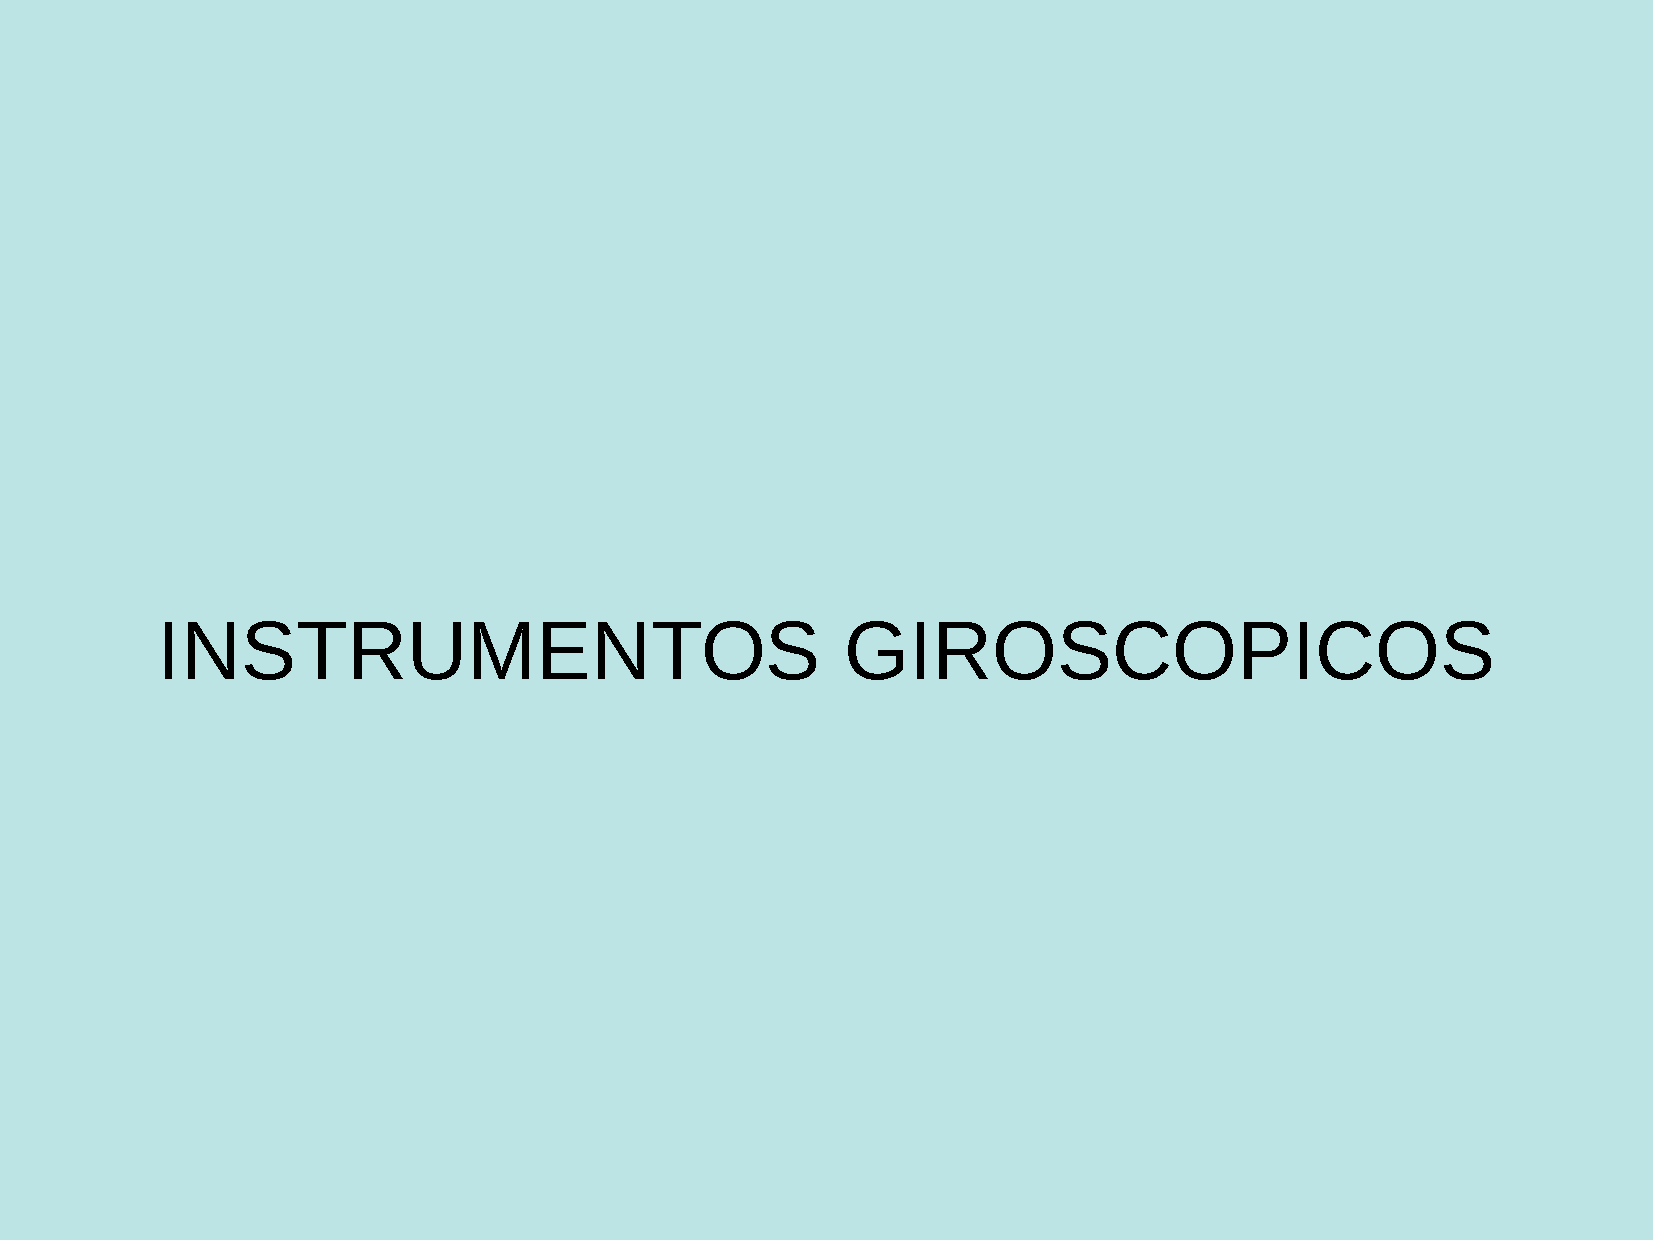
\includepdf[pages=-, %fitpaper=true,
  scale=0.80, landscape= true, offset = 0 -20,
  pagecommand={\thispagestyle{fancy}}]
  {05.instrumentos.giroscopicos/instrumentos_giroscopicos_Galeasso/01_instrumentos_2020_GIROSCOPOS.pdf}

  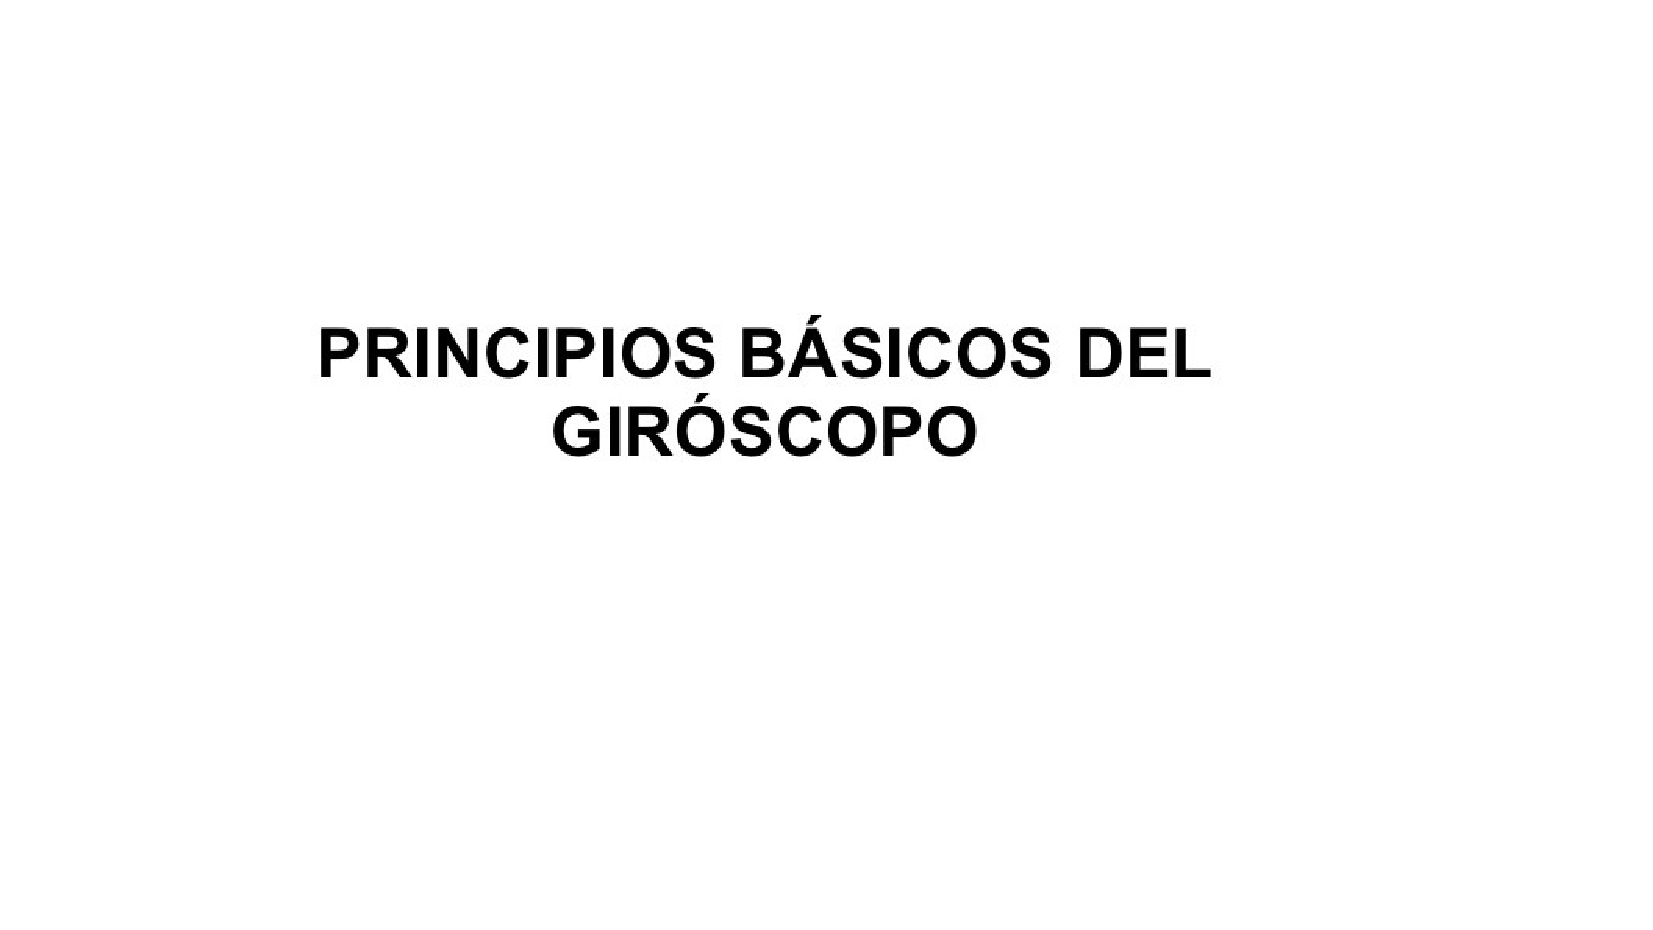
\includepdf[pages=-33, %fitpaper=true,
  scale=1, landscape= true, offset = 0 -20,
  pagecommand={\thispagestyle{fancy}}]
  {05.instrumentos.giroscopicos/instrumentos_giroscopicos_Galeasso/03_Principios_basicos_del_giroscopio.pdf}

  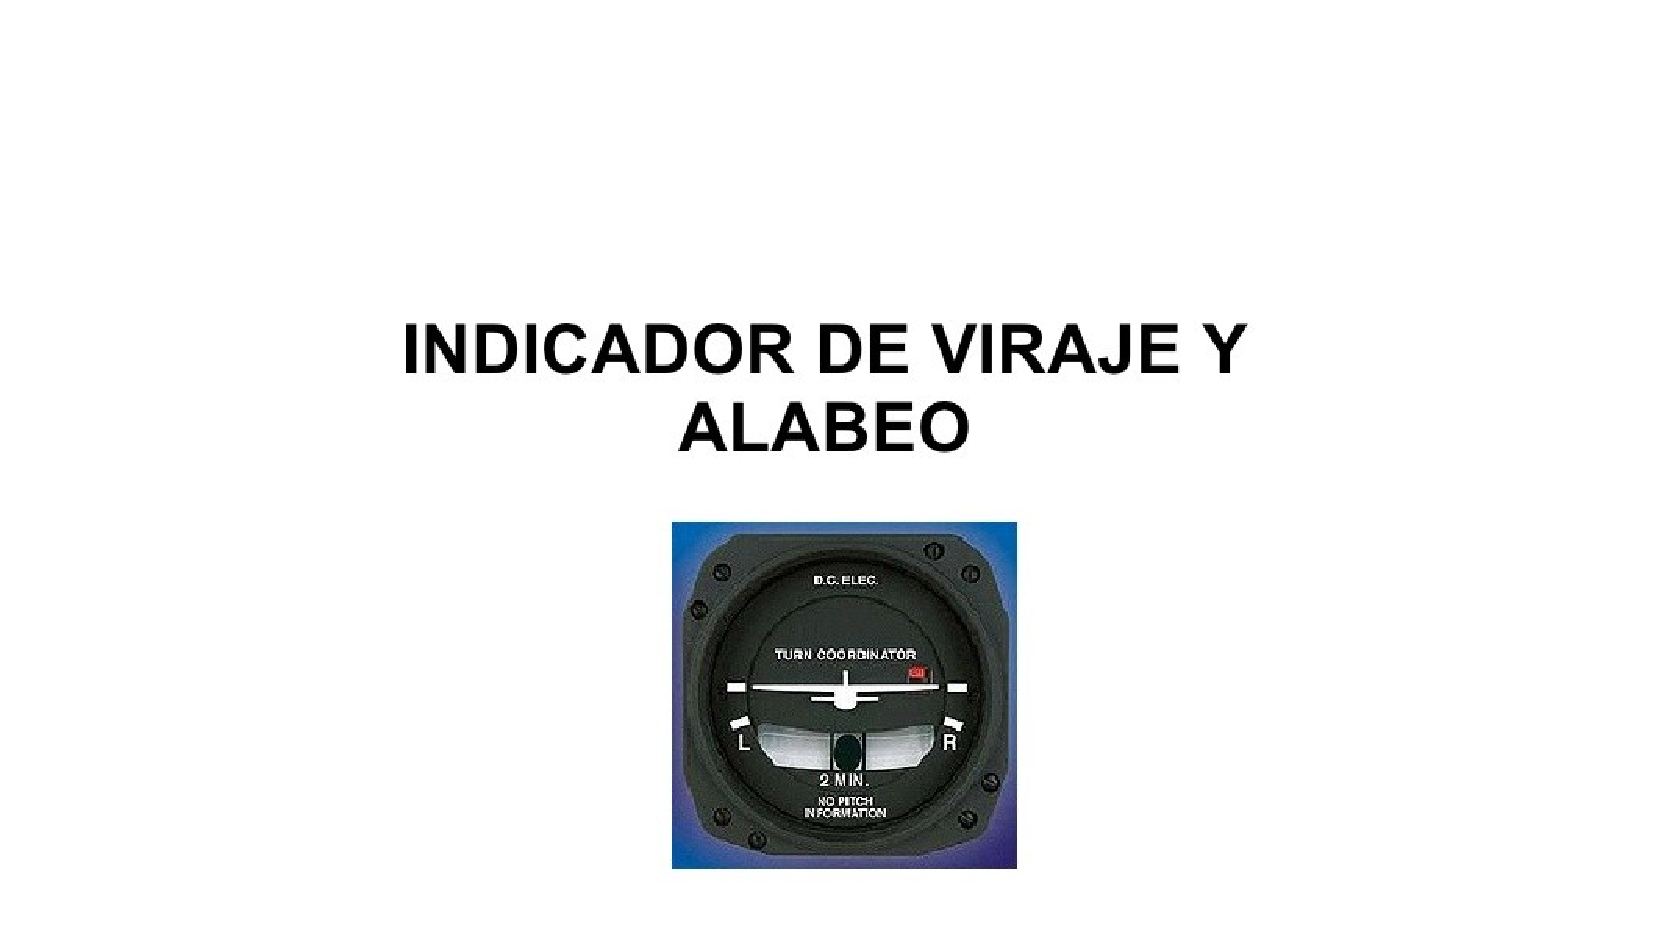
\includepdf[pages=-, %fitpaper=true,
  scale=0.9, landscape= true, offset = 0 -20,
  pagecommand={\thispagestyle{fancy}}]
  {05.instrumentos.giroscopicos/instrumentos_giroscopicos_Galeasso/04_Indicador_de_viraje_2020.pdf}

\end{landscape}

  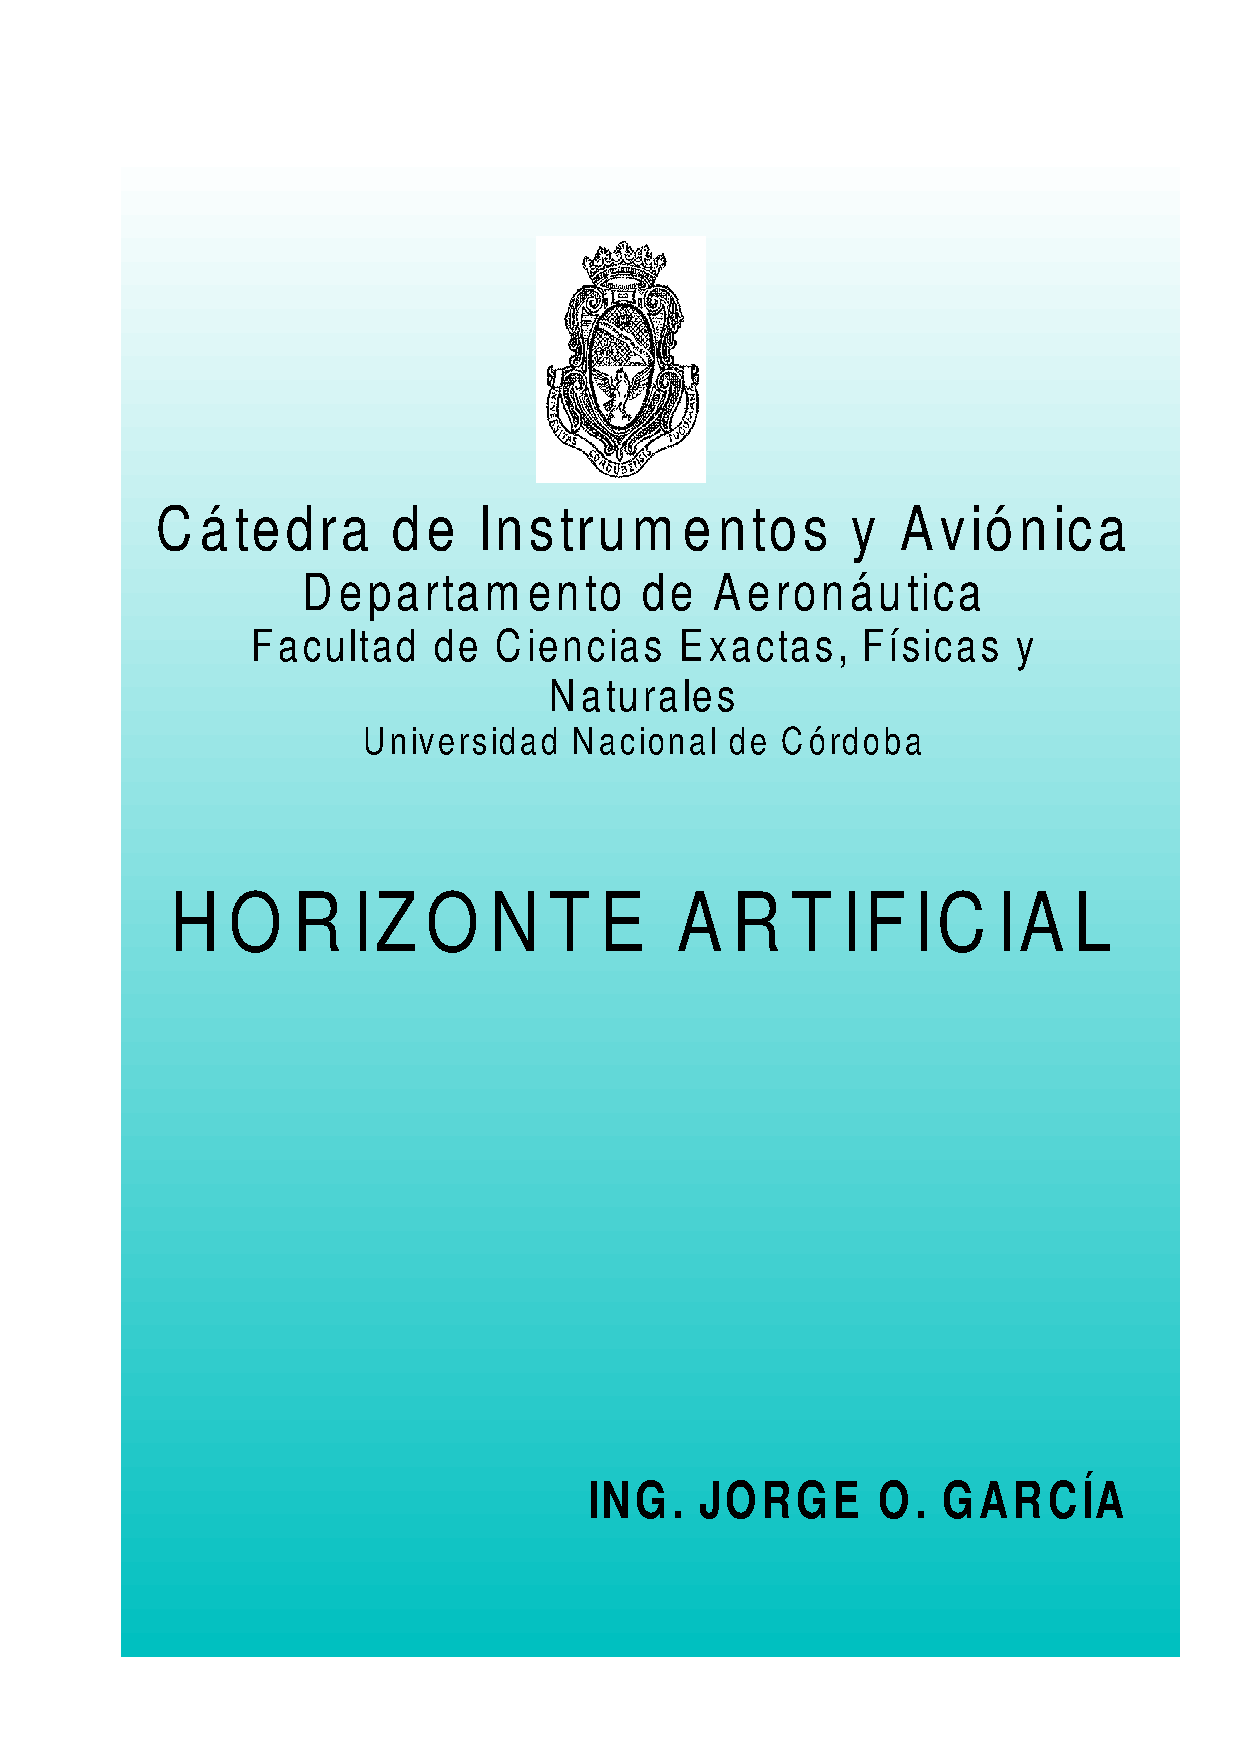
\includepdf[pages=-, %fitpaper=true,
  scale=0.9, landscape= false, offset = 0 -20,
  pagecommand={\thispagestyle{fancy}}]
  {05.instrumentos.giroscopicos/instrumentos_giroscopicos_Galeasso/05_Horizonte_artificial.pdf}

  \begin{landscape}

  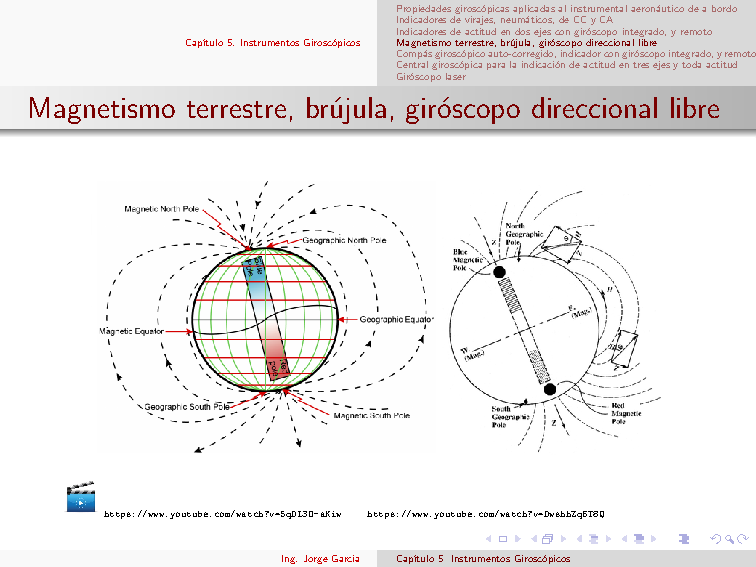
\includepdf[pages=-, %fitpaper=true,
  scale=0.8, landscape= true, offset = 0 -20,
  pagecommand={\thispagestyle{fancy}}]
  {05.instrumentos.giroscopicos/instrumentos_giroscopicos_Galeasso/06_Magnetismo_terrestre.pdf}

  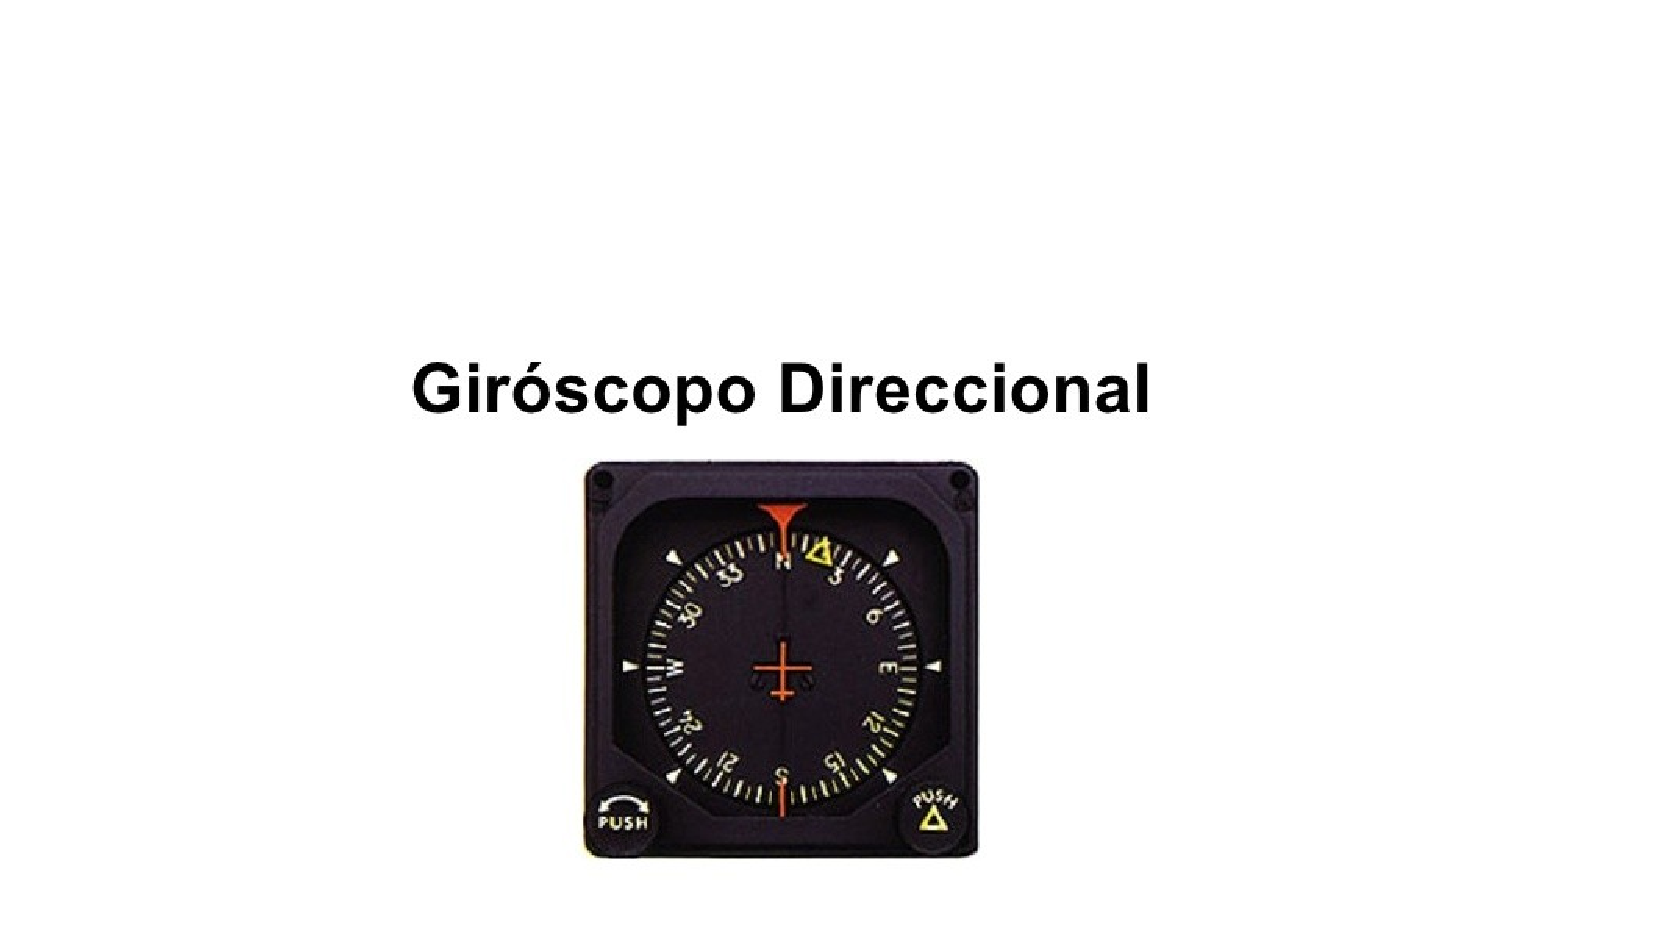
\includepdf[pages=-, %fitpaper=true,
  scale=0.9, landscape= true, offset = 0 -20,
  pagecommand={\thispagestyle{fancy}}]
  {05.instrumentos.giroscopicos/instrumentos_giroscopicos_Galeasso/07_Giroscopo_direccional.pdf}
    
  \end{landscape}


\subsection{Videos sobre instrumentos girosc\'opicos}
\label{sec:05.videos.instrumentos.giroscopicos}

  \begin{itemize}

  \item PARTE 1--                                                                     

    \begin{itemize}
    \item \href{https://www.youtube.com/watch?v=fVefWA-SV2g&feature=relmfu}{Giróscopo
        educativo }

    \item \href{https://www.youtube.com/watch?v=VXePbCxCzRA}{Giróscopo
        educativo }

    \item \href{https://www.youtube.com/watch?v=-NSUIEOPjrY}{Analogía
        traslación-rotación}
    \end{itemize}

  \item PARTE 3--

\href{https://www.youtube.com/watch?v=hVsx4XWafXg}{Video  general sobre giróscopo }

\item PARTE 4—Indicador de viraje

  \begin{itemize}
  \item \href{https://www.youtube.com/watch?v=0sRrSkSJc7w}{Indicador
      de viraje }

  \item \href{https://www.youtube.com/watch?v=a4iLtZPp_-8}{Indicador
      de viraje }
  \end{itemize}


\item PARTE 5-- Horizonte artificial

  \begin{itemize}
  \item \href{https://www.youtube.com/watch?v=f2thngd9AGI}{Horizonte
      artificial neumático}

  \item
    \href{https://www.facebook.com/1Elaviador/videos/492439044662271/}{Horizonte
      artificial }

  \item
    \href{https://www.facebook.com/Pilotviewglobal/videos/354425058384879/}{Horizonte
      artificial }

  \item \href{https://www.youtube.com/watch?v=VycrS3VYjeM}{Horizonte
      artificial}
  \end{itemize}

\item PARTE 6-- Magnetismo terrestre

\href {https://www.youtube.com/watch?v=4dDKjdj_Dvc}{Brújula magn\'etica}

% \item PARTE 7-- Compás giroscópico

% \item PARTE 8—Bases inerciales

% https://www.youtube.com/watch?v=pvRsA-bk4b4       MIG 21

% https://www.youtube.com/watch?v=LaxsIgxnf_E          MIG 23

% https://www.youtube.com/watch?v=U2JvtNbGVZc        F-104 Starfighter

\item PARTE 9--Giróscopo laser

  \begin{itemize}
  \item \href{https://www.youtube.com/watch?v=ox-LRneg1VY}{Giróscopo
      laser}

  \item \href{https://www.youtube.com/watch?v=Fk0RvzaHq_Q}{Efecto
      Sagnac}
  \end{itemize}

\end{itemize}

% \section{Introducci\'on}
% \label{sec:U05.00.introduccion}


% \section{Propiedades giroscópicas aplicadas al instrumental aeronáutico de a bordo}
% \label{sec:U05.01.propiedades.giroscopicas}


% \section{Indicadores de virajes, neumáticos, de CC y CA}
% \label{sec:U05.02.indicadores.virajes}


% \section{Indicadores de actitud en dos ejes con giróscopo integrado, y remoto}
% \label{sec:U05.03.indicadores.actitud.en.dos.ejes}

% \section{Magnetismo terrestre, brújula, giróscopo direccional libre}
% \label{sec:U05.04.magnetismo.terrestre}


% \section{Compás giroscópico auto-corregido, indicador con giróscopo integrado, y remoto}
% \label{sec:U05.05.instrumentos.giroscopicos}


% \section{Central giroscópica para la indicación de actitud en tres ejes y toda actitud}
% \label{sec:U05.06.central.giroscopica}


% \section{Giróscopo LASER}
% \label{sec:U06.07.giroscopo.laser}

